\documentclass[11pt,a4paper]{article}

% --- Layout ---
\usepackage[margin=1in]{geometry}
\usepackage{setspace}
\setstretch{1.08}

% --- Encoding & language ---
\usepackage[utf8]{inputenc}
\usepackage[T1]{fontenc}
\usepackage{lmodern}
\usepackage{textcomp}
\usepackage[english]{babel}

% --- Math ---
\usepackage{amsmath, amssymb, amsthm}
\usepackage{mathtools}

% --- Figures & tables ---
\usepackage{graphicx}
\graphicspath{{figures/}}
\usepackage{booktabs}
\usepackage{array}
\usepackage{caption}
\captionsetup{font=small,labelfont=bf,format=plain,justification=justified}
\usepackage{float}

% --- Lists & code ---
\usepackage{enumitem}
\setlist{nosep}
\usepackage{verbatim}

% --- References ---
\usepackage[numbers,square,sort&compress]{natbib}
\bibliographystyle{plainnat}

% --- Links ---
\usepackage[hidelinks,breaklinks=true]{hyperref}
\usepackage{url}

% --- Footnotes/macros ---
\newcommand{\AOD}{\text{AOD}}
\newcommand{\SZA}{\text{SZA}}
\newcommand{\tauR}{\tau_R}
\newcommand{\tauM}{\tau_{\text{Mie}}}
\newcommand{\tauO}{\tau_{\mathrm{O_3}}}
\newcommand{\tautotal}{\tau_{\text{total}}}
\DeclareMathOperator{\trap}{trap}

% --- Title ---
\title{An Operational, Physics-Motivated Framework for\\
Sunset Glow Prediction over the Continental United States}
\author{Nick Zhu \\ \small\texttt{zhuxyparzival@gmail.com}}
\date{\today\\\small Working draft v0.4 --- arxiv preprint target}

\begin{document}
\maketitle

\begin{abstract}
Vivid sunset and sunrise glows---colloquially ``fire clouds'' in Chinese (\textit{huoshaoyun})---arise from a narrow set of atmospheric conditions: mid- to high-level clouds illuminated by low-angle sunlight that has traversed a long atmospheric path, with the troposphere clean enough to deliver ``unadulterated'' red light to the cloud canvas. Existing commercial prediction services (SunsetWx, Sunsethue) score these conditions with weighted-sum combinations of meteorological variables, treating necessary conditions (such as the presence of mid- or high-level clouds) as substitutable for other favorable factors. We show this produces substantial false positives: in an end-to-end run over Washington State's Olympic Peninsula at sunset on 20 May 2026, a weighted-sum predictor returned probabilities of 0.625--0.631 uniformly across all 180 cells of a 0.1\textdegree{}-resolution grid despite mid- and high-level cloud coverage of zero. We propose a two-layer scoring architecture in which physically necessary conditions act as multiplicative gates and enhancement variables modulate the result. The framework incorporates ozone Chappuis-band absorption---recently shown by \citet{lange2023revisiting} to dominate twilight blue color at low solar elevations---as an explicit pathway alongside Rayleigh and Mie scattering. We implement the framework as an open-source Python package consuming NOAA's High Resolution Rapid Refresh (HRRR) numerical weather prediction data, and present a preliminary case study comparison: the proposed gate $\times$ modifier scheme correctly returns zero across the Olympic Peninsula bounding box, where weighted-sum scoring fails. Full validation against citizen-science ground truth is identified as future work.

\medskip
\noindent\textbf{Keywords:} atmospheric optics; twilight color; sunset prediction; numerical weather prediction; operational forecasting; Rayleigh scattering; Mie scattering; ozone Chappuis absorption.
\end{abstract}

\section{Introduction}

\subsection{The Phenomenon}

A ``sunset glow'' or ``afterglow''---the brief reddening of mid- and high-level clouds in the western sky around sunset---is among the most widely photographed atmospheric phenomena, with significant cultural resonance in many languages (Chinese \textit{huoshaoyun}, English ``afterglow'', Spanish \textit{arrebol}). Beyond aesthetic interest, the conditions producing a vivid sunset glow integrate several distinct branches of atmospheric science: scattering theory (Rayleigh and Mie regimes), gas-phase absorption (ozone Chappuis band), cloud microphysics (the boundary layer's role in attenuation), and the geometry of low-elevation solar paths.

Knowing when and where a sunset glow will occur has practical value for landscape photographers and amateur astronomers, but the underlying integration of variables makes it a useful pedagogical case for atmospheric optics. The problem has the unusual property that necessary conditions (a cloud canvas above the boundary layer, low-angle illumination, a clean troposphere) are difficult to substitute one for another: no amount of cloud will help if the sun is overhead, no amount of solar geometry will help in dense overcast.

\subsection{Existing Approaches}

Three public services currently offer sunset color predictions for North America: SunsetWx, a Penn State--origin model using NOAA Global Forecast System (GFS) data with a 20-factor weighted scoring algorithm \citep{forecastingbeauty2015}; Sunsethue, an independent service that publishes cloud-cover, altitude, humidity, and air-quality thresholds in narrative form on its blog; and Skyfire, a closed-source feature of the PhotoPills planning application. None of these services has published a peer-reviewed methodology paper, released scoring weights, or provided systematic validation against ground truth.

Peer-reviewed research on twilight color has focused on the optical mechanism rather than operational prediction. Foundational works include \citet{strutt1871scattering}'s derivation of the $\lambda^{-4}$ molecular scattering dependence, \citet{mie1908beitrage}'s treatment of arbitrary-sized particle scattering, and \citet{hulburt1953explanation}'s early recognition that ozone absorption contributes substantially to sky color. Operational synthesis includes \citet{corfidi2014colors}'s summary for the NOAA Storm Prediction Center, which provides the most authoritative qualitative account of which clouds redden and why.

Recent quantitative work has refined the textbook picture. \citet{lee2003purple} combined spectral measurements over multiple seasons with radiative transfer modeling to show that twilight's ``purple light'' cannot be attributed to stratospheric aerosols alone: both tropospheric and stratospheric scattering and extinction are required. \citet{lange2023revisiting} revisited the canonical question of why the sky is blue, demonstrating with the SCIATRAN radiative transfer model that ozone Chappuis-band absorption, not Rayleigh scattering, dominates sky blue color at high solar zenith angles: at total ozone column 300\,DU with zenith viewing geometry, ozone contributes 66\% of the blue color and Rayleigh only 34\%.

The gap addressed by the present work lies between these two strands of literature. Existing operational prediction tools lack a physics-rigorous foundation; peer-reviewed optics literature has not been translated into a deployable forecasting framework.

\subsection{Contributions}

This paper contributes:
\begin{enumerate}
\item An explicit catalog of necessary versus enhancing conditions for sunset glow formation, grounded in current peer-reviewed atmospheric optics literature (Section~\ref{sec:theory}).
\item A two-layer \emph{gate $\times$ modifier} scoring architecture that respects the multiplicatively-gated nature of necessary conditions, avoiding a class of false positives produced by weighted-sum scoring (Section~\ref{sec:methodology}).
\item To the authors' knowledge, the first published prediction framework to incorporate ozone Chappuis-band absorption as an explicit factor, building directly on \citet{lange2023revisiting} (Sections~\ref{sec:atmoptics} and~\ref{sec:rules}).
\item An open-source Python implementation consuming NOAA HRRR data, with end-to-end reproducibility (Section~\ref{sec:implementation}, code at \texttt{https://github.com/NickZhuxy/firecloud-forecast}).
\item A preliminary case study on the Olympic Peninsula demonstrating the false-positive pathology of additive scoring and motivating the gate $\times$ modifier alternative (Section~\ref{sec:casestudy}).
\end{enumerate}

\subsection{Outline}

Section~\ref{sec:theory} develops the theoretical background spanning atmospheric optics, solar geometry, cloud physics, and aerosol effects, concluding with a synthesis of necessary versus enhancing conditions. Section~\ref{sec:methodology} defines the methodology: data sources, feature derivation, scoring rule design, and the gate $\times$ modifier architecture. Section~\ref{sec:implementation} describes the software implementation. Section~\ref{sec:casestudy} presents a preliminary case study. Section~\ref{sec:discussion} discusses implications and acknowledges limitations. Section~\ref{sec:conclusion} concludes with planned future work, including a citizen-science validation pipeline and a planned extension to global coverage.

\section{Theoretical Background}
\label{sec:theory}

\subsection{Atmospheric Optics: Three Mechanisms of Selective Extinction}
\label{sec:atmoptics}

The color of a sunset glow is the surviving signature of selective light extinction along the long optical path from the sun to a high-altitude cloud surface. Three independent mechanisms contribute, in order of decreasing wavelength selectivity: molecular Rayleigh scattering, gas-phase Chappuis-band ozone absorption, and aerosol Mie scattering. We treat each in turn and combine them via the Beer--Lambert law.

\subsubsection{Rayleigh Scattering}

For air molecules with diameters far smaller than the wavelength of visible light ($D \ll \lambda$), the scattering cross section follows \citet{strutt1871scattering}'s classical result:
\begin{equation}
\sigma_R(\lambda) = \frac{8 \pi^3 (n^2 - 1)^2}{3 N^2 \lambda^4}
\label{eq:rayleigh}
\end{equation}
where $n$ is the refractive index of air and $N$ is the molecular number density. The defining feature is the $\lambda^{-4}$ dependence: violet light at 400\,nm has a scattering cross section approximately $(700/400)^4 \approx 9.4$ times that of red light at 700\,nm. \citet{bodhaine1999rayleigh} provide a precise treatment incorporating the King correction factor (approximately 1.05, reflecting molecular anisotropy) and refractive-index dispersion; these refinements add roughly 5\% to the leading $1/\lambda^4$ term and we do not develop them here.

\subsubsection{Mie Scattering}

For particles whose size is comparable to the wavelength of light, the Rayleigh approximation breaks down and the full \citet{mie1908beitrage} solution to electromagnetic scattering by a sphere is required. The relevant non-dimensional parameter is the size parameter
\begin{equation}
x = \frac{2 \pi r}{\lambda}
\label{eq:sizeparam}
\end{equation}
with three regimes:
\begin{itemize}
\item $x \ll 1$: Rayleigh limit, $\sigma \propto \lambda^{-4}$ as above.
\item $x \sim 1$: Mie regime, oscillatory dependence on $\lambda$ with overall near-grayness.
\item $x \gg 1$: geometric optics limit.
\end{itemize}

For visible light ($\lambda \in [0.4, 0.7]\,\mu\mathrm{m}$) and typical tropospheric aerosol radii ($r \in [0.05, 0.5]\,\mu\mathrm{m}$, corresponding to particle diameters $D \in [0.1, 1.0]\,\mu\mathrm{m}$), the size parameter $x$ falls in the range 1--10. This places anthropogenic pollution, mineral dust, and most biomass-burning aerosols squarely in the Mie oscillation regime. \citet[\S22.4]{stull2017practical} summarizes the practical implications in tabular form:

\begin{table}[H]
\centering
\small
\begin{tabular}{lll l}
\toprule
$D/\lambda$ & Diameter & Source & Scattering type \\
\midrule
$< 1$ & 0.0001--0.001 $\mu$m & Air molecules & Rayleigh \\
$\approx 1$ & 0.01--1.0 $\mu$m & Aerosols, smoke, PM2.5 & Mie \\
$> 1$ & 10--100 $\mu$m & Cloud droplets & Geometric \\
\bottomrule
\end{tabular}
\caption{Scattering regime by particle size relative to wavelength, after \citet[\S22.4]{stull2017practical}.}
\label{tab:stull}
\end{table}

The consequence for sunset color is that tropospheric pollution, far from enhancing red hues, \emph{attenuates the full visible spectrum nearly uniformly}, producing the pale, washed-out sunsets characteristic of urban haze. This is the physical mechanism behind \citet{corfidi2014colors}'s operational observation that ``clean air is, in fact, the main ingredient common to brightly colored sunrises and sunsets.''

\subsubsection{Ozone Chappuis Absorption}

Ozone has a broad, weak absorption band in the 500--700\,nm range known as the Chappuis band, with peak absorption near 600\,nm. At solar zenith angles approaching $90^\circ$ the optical path through the stratospheric ozone layer is approximately 30 times longer than at solar noon, so Chappuis absorption becomes correspondingly more important at sunset.

\citet{lange2023revisiting} used the SCIATRAN radiative transfer model to quantify the relative contributions of Rayleigh scattering versus ozone Chappuis absorption to the perceived blueness of the twilight sky. For 300\,DU total ozone column at solar zenith angle $90^\circ$ and zenith viewing, they find ozone contributes 66\% and Rayleigh 34\% to the chromaticity displacement. The contribution varies systematically with total ozone column: 60\% at 240\,DU, 76\% at 500\,DU. Their result confirms a long-standing single-scattering estimate by \citet{hulburt1953explanation} using modern multi-scattering radiative transfer. This finding modifies the textbook picture in which Rayleigh scattering is the sole explanation for sky blue---and by extension, contributes to the late-stage reddening of sunset glow by removing residual orange-yellow wavelengths in transit through the ozone layer.

\subsubsection{Combined Extinction}

The three mechanisms combine additively in optical depth. For sunlight along a path of geometric length $L$, the surviving spectral irradiance is
\begin{equation}
\frac{I(\lambda)}{I_0(\lambda)} = e^{-\tautotal(\lambda)}
\label{eq:beer}
\end{equation}
with
\begin{equation}
\tautotal(\lambda) = \tauR(\lambda) + \tauM(\lambda) + \tauO(\lambda)
\label{eq:tausum}
\end{equation}
where each term integrates the corresponding extinction coefficient along the path. At low solar elevation, the path length is dominated by horizontal transit through the lower atmosphere (Section~\ref{sec:solargeometry}). Figure~\ref{fig:extinction} illustrates the wavelength-resolved contributions at $\SZA = 90^\circ$ using standard atmospheric approximations: Rayleigh dominates the blue end and decays steeply with wavelength; Mie is nearly flat; Chappuis forms a smaller but distinct hump around 600\,nm. The cumulative effect on transmission shows orders-of-magnitude attenuation across the visible band, with only the deep red surviving at substantial fraction---the physical answer to why sunsets are red.

\begin{figure}[H]
\centering
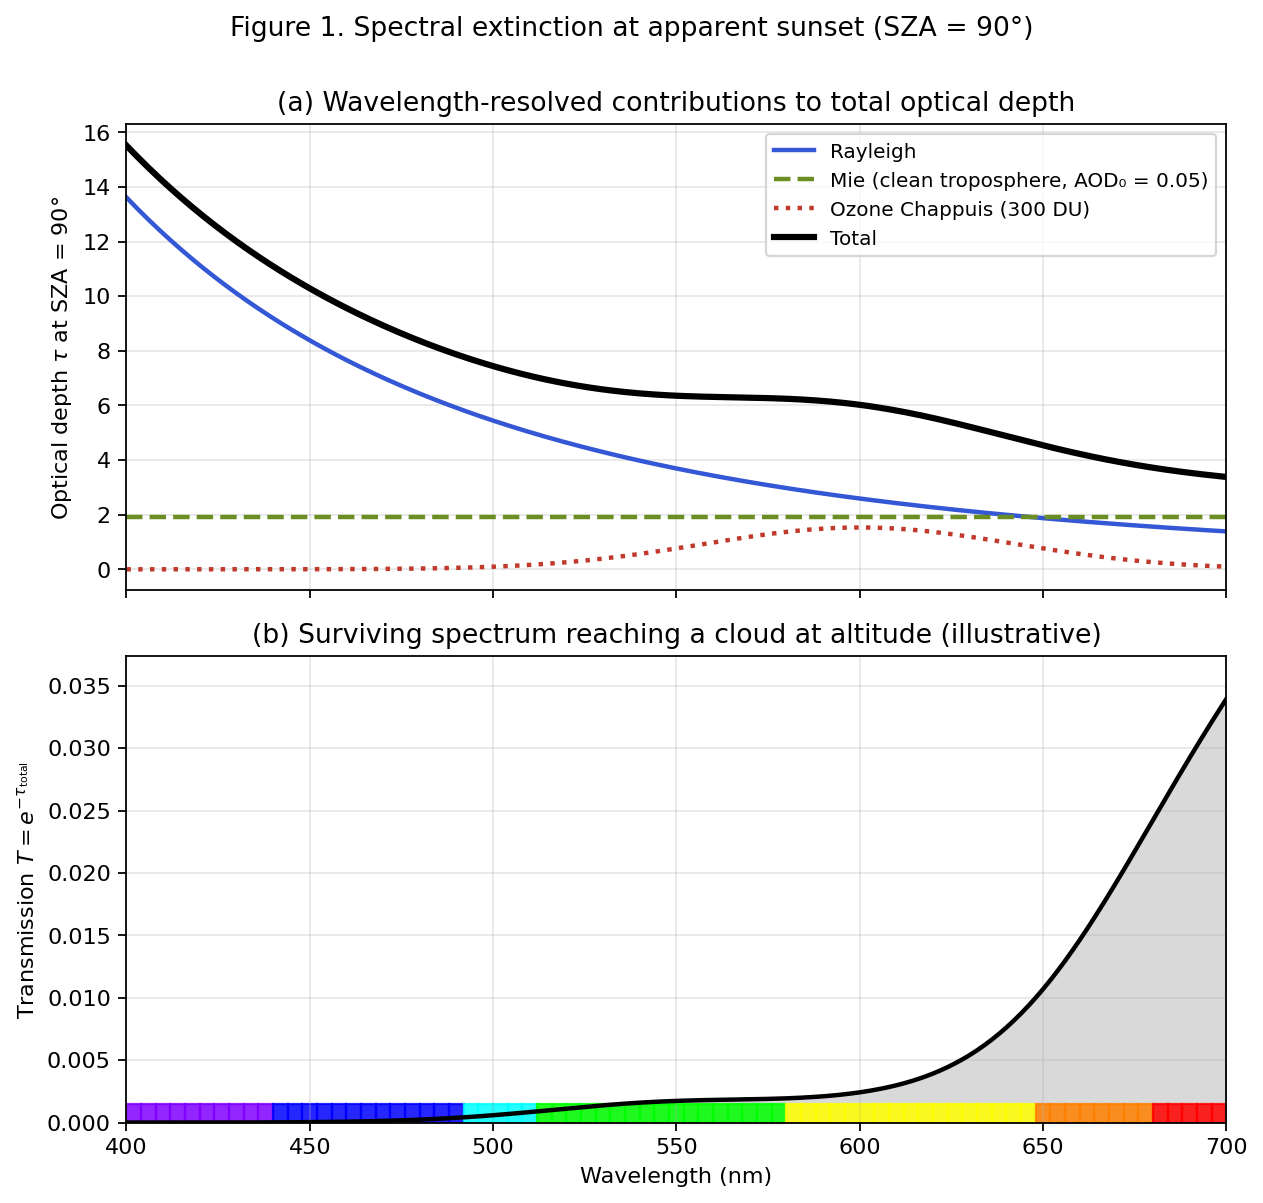
\includegraphics[width=0.85\linewidth]{fig1_extinction_spectrum.png}
\caption{Spectral extinction at apparent sunset ($\SZA = 90^\circ$). \textbf{Top:} Rayleigh (Bodhaine-form), Mie (clean-troposphere $\AOD_0 = 0.05$), and ozone Chappuis (300\,DU, Gaussian approximation around 600\,nm) contributions to total optical depth, scaled by Kasten--Young air mass $m = 38$. \textbf{Bottom:} surviving transmission $T = e^{-\tautotal}$; the color band along the bottom encodes wavelength as a perceptual color reference. Values are illustrative; for camera-ready figures a full radiative transfer model is recommended.}
\label{fig:extinction}
\end{figure}

\subsection{Solar Geometry: Air Mass and the Twilight Window}
\label{sec:solargeometry}

The extinction integrals of Section~\ref{sec:atmoptics} take a geometric path length as input. At low solar elevations the path length is dominated by horizontal transit through the lower atmosphere; this section makes the corresponding geometry quantitative and connects it to the duration of cloud illumination after sunset.

\subsubsection{Solar Elevation and Twilight}

Let the solar elevation angle $\alpha$ denote the angle of the sun's center above the local horizontal plane (with the solar zenith angle $\SZA = 90^\circ - \alpha$). Atmospheric refraction raises the sun's apparent position by approximately $34'$ near the horizon, so the \emph{apparent} sunset (when the sun's upper limb appears tangent to the horizon) occurs when the geometric elevation is approximately $-0.83^\circ$, accounting for the refractive lift and the sun's apparent angular radius of $0.27^\circ$.

By international convention, the twilight intervals are defined in terms of geometric solar elevation:
\begin{itemize}
\item \textbf{Civil twilight}: $-6^\circ \leq \alpha \leq 0^\circ$. The brighter planets and stars become visible.
\item \textbf{Nautical twilight}: $-12^\circ \leq \alpha \leq -6^\circ$. The horizon line remains distinguishable.
\item \textbf{Astronomical twilight}: $-18^\circ \leq \alpha \leq -12^\circ$. Residual scattered light persists at the zenith but is undetectable to the naked eye.
\end{itemize}

The visual sunset glow phenomenon of interest in this paper occupies approximately $\alpha \in [-6^\circ, +5^\circ]$, straddling apparent sunset and extending through most of civil twilight.

\subsubsection{Optical Air Mass}

The \emph{relative optical air mass} $m$ is defined as the ratio of the slant atmospheric path length to the vertical path length at the same location. In the plane-parallel approximation, valid for $\SZA \lesssim 75^\circ$,
\begin{equation}
m \approx \sec(\SZA) = \frac{1}{\cos(\SZA)}.
\end{equation}
Near the horizon, $\sec(\SZA)$ diverges and the plane-parallel approximation fails. The current standard treatment is the \citet{kasten1989airmass} formula, derived from numerical integration over the ISO Standard Atmosphere (1972) profile up to 84\,km:
\begin{equation}
m(\SZA) = \frac{1}{\cos(\SZA) + 0.50572 \,(96.07995 - \SZA)^{-1.6364}},
\label{eq:kastenyoung}
\end{equation}
with $\SZA$ in degrees. Representative values:

\begin{table}[H]
\centering
\small
\begin{tabular}{rrr}
\toprule
$\alpha$ & $\SZA$ & $m$ \\
\midrule
$90^\circ$ (zenith) & $0^\circ$ & 1.00 \\
$30^\circ$ & $60^\circ$ & 2.00 \\
$10^\circ$ & $80^\circ$ & 5.60 \\
$5^\circ$ (early sunset glow) & $85^\circ$ & 10.4 \\
$1^\circ$ & $89^\circ$ & 27 \\
$0^\circ$ (apparent sunset) & $90^\circ$ & 38 \\
\bottomrule
\end{tabular}
\caption{Relative optical air mass at representative solar elevations, computed from Eq.~\ref{eq:kastenyoung}.}
\label{tab:airmass}
\end{table}

The path length at apparent sunset is approximately 38 times the vertical path length at zenith. The wavelength-resolved extinction integrals of Section~\ref{sec:atmoptics} thus accumulate over a path 38 times longer than at solar noon, which is the geometric origin of the large color shift that distinguishes sunset light from midday light.

\subsubsection{Horizon Depression Angle}
\label{sec:horizondepression}

For a cloud at altitude $h$ above an observer at sea level, define the \emph{horizon depression angle} $d(h)$ as the geometric solar elevation below the observer's horizon at which the cloud first loses direct illumination by the sun. With Earth radius $R_\oplus = 6371$\,km,
\begin{equation}
d(h) = \arccos\left(\frac{R_\oplus}{R_\oplus + h}\right), \qquad d(h) \approx \sqrt{\frac{2 h}{R_\oplus}} \text{ (small-angle)}.
\label{eq:depression}
\end{equation}

Figure~\ref{fig:horizon} plots $d(h)$ and the corresponding direct-illumination time window $\Delta t(h) = 2 d(h) / |d\alpha/dt|$ across the relevant altitude range, with WMO altitude bands shaded for reference. The asymmetry between high and low clouds is striking: low stratus or stratocumulus at 1\,km altitude loses direct sunlight within minutes of apparent sunset; cirrus at 10\,km remains directly lit for nearly twenty minutes more. Indirect illumination by multiply-scattered light extends the visual sunset glow phenomenon further still---qualitative reports of high cirrus visibly illuminated up to 30 minutes after sunset are consistent with the geometric upper bound modulo a few minutes of secondary scattering.

\begin{figure}[H]
\centering
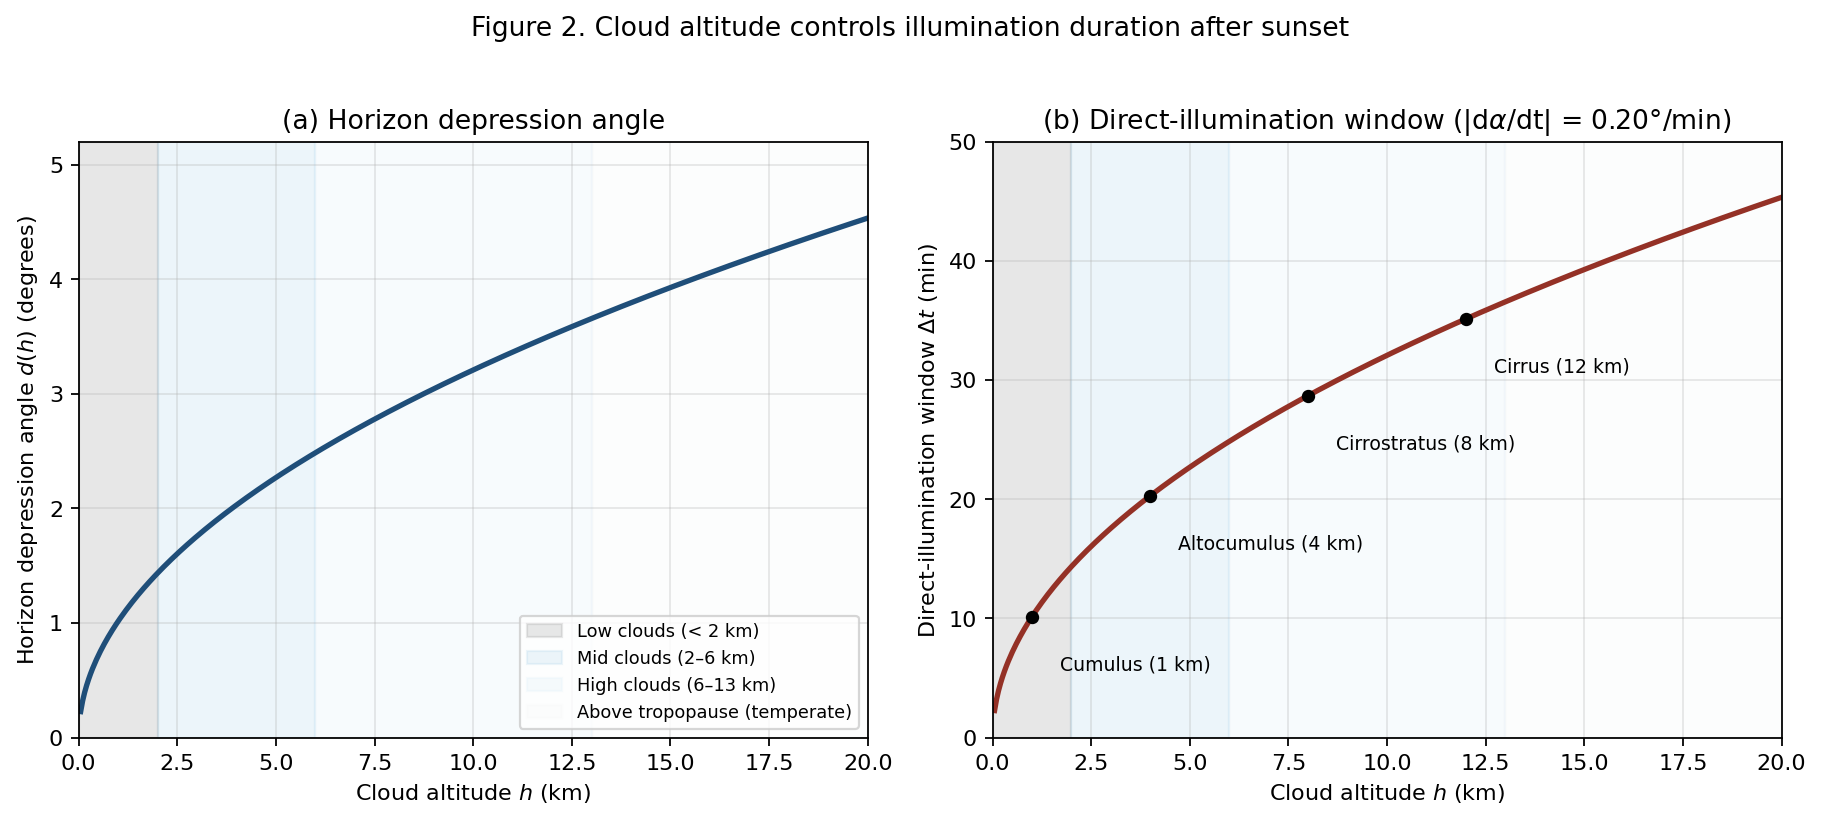
\includegraphics[width=0.95\linewidth]{fig2_horizon_depression.png}
\caption{Cloud altitude controls illumination duration after sunset. \textbf{Left:} horizon depression angle $d(h) = \arccos(R_\oplus / (R_\oplus + h))$ as a function of cloud altitude $h$. \textbf{Right:} direct-illumination time window $\Delta t(h) = 2 d(h) / |d\alpha/dt|$ from apparent sunset, using a representative mid-latitude solar elevation rate $|d\alpha/dt| = 0.20^\circ/$min. Annotations show typical cloud-type altitudes. WMO three-tier altitude bands (low, mid, high) shaded in both panels.}
\label{fig:horizon}
\end{figure}

\subsubsection{A Parabolic Reformulation in Flat Coordinates}
\label{sec:parabola}

The trigonometric apparatus above becomes more tractable for forecasting practice in a flattened coordinate system. Define $l = R_\oplus \theta$ as arc length along Earth's surface and $h$ as altitude above the surface. In these coordinates, surfaces of constant altitude become horizontal lines, but a straight sunlight ray that grazes Earth's surface tangentially at the origin acquires a quadratic profile. Using $r = R_\oplus + h = R_\oplus / \cos\theta$ and expanding to second order in $\theta = l / R_\oplus$,
\begin{equation}
h(l) \approx \frac{l^2}{2 R_\oplus},
\label{eq:parabola}
\end{equation}
with relative error $\sim (l / R_\oplus)^4$ that is negligible for the few-hundred-kilometer scales of sunset light propagation. A ray that grazes the surface at $l = l_0$ at altitude $h_0$ takes the translated form
\begin{equation}
h(l) = \frac{(l - l_0)^2}{2 R_\oplus} + h_0.
\label{eq:parabola_translated}
\end{equation}

The flattening trades curvilinear Earth geometry for parabolic light paths but eliminates trigonometric functions and converts rotations (Earth's rotation, which changes solar zenith angle) into translations. For a level cloud base at altitude $h_{CB}$, the constraint $h(l) = h_{CB}$ together with Eq.~\ref{eq:parabola} yields the maximum surface distance from an observer at which sunlight can graze Earth and just reach the underside of the cloud:
\begin{equation}
|l|_{\max} = 2 \sqrt{2 R_\oplus \, h_{CB}}.
\label{eq:max_penetration}
\end{equation}

Equation~\ref{eq:max_penetration} is a closed-form upper bound on the horizontal range over which a fire cloud can form for a given cloud base altitude. Representative values: $h_{CB} = 2$~km gives $|l|_{\max} \approx 319$~km; $h_{CB} = 5$~km gives 505~km; $h_{CB} = 10$~km gives 714~km. For an observer to see a fire cloud, a candidate cloud's near boundary must lie within this distance along the sunset direction.

\subsubsection{Fire-Cloud Spatiotemporal Triangle}
\label{sec:triangle}

Combining the parabolic geometry of Section~\ref{sec:parabola} with Earth's rotation produces a closed-form characterization of when and where fire-cloud illumination is geometrically possible. For an observer at the origin and a flat-bottom cloud layer at altitude $h_{CB}$, define $v = -R_\oplus \, d\phi/dt$ as the linear velocity at which the sunset terminator moves along the sunset direction (with $\phi$ the solar elevation). Two boundary rays delimit the illuminated region at any instant $t$ after the observer's apparent sunset:

\begin{itemize}
\item The \emph{far boundary} $l_f(t)$ is set by Earth's shadow---rays graze the surface tangentially. With $L \equiv \sqrt{2 R_\oplus h_{CB}}$,
\begin{equation}
l_f(t) = -L + v t.
\end{equation}
\item The \emph{near boundary} $l_n(t)$ is set by the cloud's own edge blocking light from below:
\begin{equation}
l_n(t) = \begin{cases} 2 v t, & t \leq 0, \\ 0, & t > 0. \end{cases}
\end{equation}
\end{itemize}

The two boundaries coincide at $(t, l) = (-L/v, -2L)$ and again at $(L/v, 0)$. Between these points, the illuminated horizontal extent at time $t$ is $\Delta l(t) = l_n(t) - l_f(t)$, defining a triangular region in the $(t, l)$ plane (Figure~\ref{fig:triangle}). The triangle encodes several operational consequences for fire-cloud prediction:

\begin{enumerate}
\item For a flat-bottom layer cloud, the local fire cloud at the observer's zenith \emph{always occurs after apparent sunset (or before apparent sunrise)}, never simultaneously.
\item Higher cloud base $h_{CB}$ enlarges both axes of the triangle ($\propto \sqrt{h_{CB}}$): a fire cloud reaches farther and lasts longer.
\item The longest fire-cloud duration at any single fixed location occurs near the cloud's own boundary, not deep inside the cloud sheet.
\item For an evening fire cloud, illumination begins at the innermost edge of the cloud relative to the observer and propagates outward along the sunset direction; the morning case is time-reversed.
\item A fire cloud may still be visible when the cloud's sun-direction boundary is below the observer's local horizon, but only if the boundary is sufficiently distant.
\end{enumerate}

\begin{figure}[H]
\centering
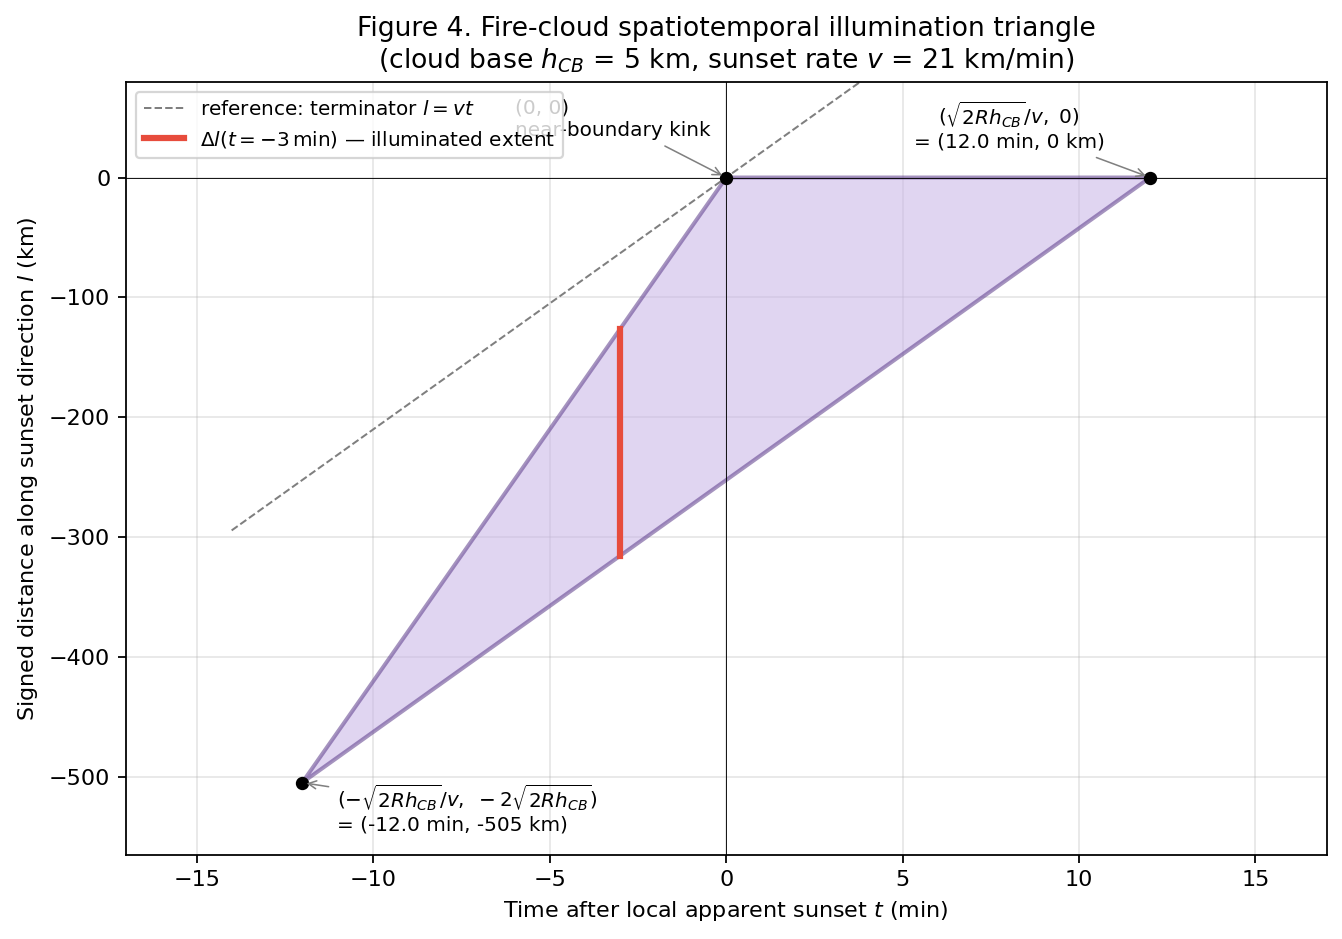
\includegraphics[width=0.85\linewidth]{fig4_spatiotemporal_triangle.png}
\caption{Fire-cloud spatiotemporal illumination triangle for a flat-bottom cloud layer with base $h_{CB}$. The shaded triangle is the set of $(t, l)$ pairs for which direct sunlight can illuminate the cloud base. The far boundary (lower edge) is set by Earth's shadow; the near boundary (upper edges) is set by the cloud's own edge for $t \leq 0$ and by the observer's zenith for $t > 0$. The horizontal red bar marks the illuminated extent at a representative instant $t = -3$~min. The dashed reference line is the geometric sunset terminator $l = vt$. Parameters: $h_{CB} = 5$~km, sunset rate $v = 21$~km/min.}
\label{fig:triangle}
\end{figure}

\subsection{Cloud Physics: Altitude, Type, and the Planetary Boundary Layer}

The geometric argument of Section~\ref{sec:horizondepression} is one of three independent mechanisms that together explain why mid- and high-level clouds dominate the sunset glow phenomenon while low clouds rarely produce vivid color. This section develops the remaining two mechanisms---boundary-layer attenuation of incoming sunlight and the high optical thickness of low water clouds---after summarizing the standard cloud classification used in the literature and in NOAA's HRRR output.

\subsubsection{Cloud Classification by Altitude}

The \citet{wmo_cloud_atlas} partitions tropospheric clouds into three altitude tiers, with characteristic genera in each. For temperate latitudes:

\begin{table}[H]
\centering
\small
\begin{tabular}{lcccc}
\toprule
Tier & Cloud base altitude & Principal genera & Composition & Optical thickness $\tau_c$ \\
\midrule
High & 5--13\,km & Cirrus (Ci), Cirrocumulus (Cc), Cirrostratus (Cs) & Ice crystals & Typically $< 1$ \\
Middle & 2--6\,km & Altocumulus (Ac), Altostratus (As), Nimbostratus (Ns) & Mixed water and ice & $\sim 1$--$10$ \\
Low & $< 2$\,km & Stratus (St), Stratocumulus (Sc), Cumulus (Cu) & Water droplets & Often $> 10$ \\
\bottomrule
\end{tabular}
\caption{WMO cloud classification by altitude (temperate latitudes). Altitudes shift with latitude; the NOAA HRRR cloud-cover variables HCDC/MCDC/LCDC correspond broadly to the three tiers although precise layer boundaries differ.}
\label{tab:wmo}
\end{table}

\subsubsection{The Planetary Boundary Layer}

The \emph{planetary boundary layer} (PBL) is the lowest portion of the troposphere where the surface exerts a direct influence on the atmosphere through frictional drag and surface heat flux, driving turbulent mixing of momentum, heat, moisture, and trace constituents. Typical daytime PBL depths over continental midlatitudes are 1--2\,km, rising to 3\,km in summer over hot dry surfaces and collapsing to a few hundred meters at night. After sunset a \emph{residual layer} containing the day's accumulated aerosol burden persists at roughly the daytime PBL depth for several hours before mixing with the nocturnal stable layer.

The PBL contains the great majority of tropospheric aerosols, water vapor, and anthropogenic pollutants. As a consequence, light traversing horizontally through the PBL---as low-angle sunset light must---encounters a far greater integrated extinction than light traversing only the free troposphere above.

\subsubsection{Three Mechanisms for Cloud Altitude Selectivity}

The dominance of mid- and high-level clouds in sunset glow formation results from three independent mechanisms acting in concert.

\paragraph{Mechanism 1: Geometric illumination window} Developed in Section~\ref{sec:horizondepression}. A cloud at altitude $h$ remains directly illuminated for a time window scaling as $\sqrt{h}$ around apparent sunset. Low clouds at 1\,km altitude have direct-illumination windows of order minutes; high cirrus at 10--15\,km has windows approaching half an hour.

\paragraph{Mechanism 2: Boundary-layer attenuation of incoming sunlight} At low solar elevation the optical path from sun to a cloud at altitude $h$ traverses substantial horizontal distance through the PBL, encountering boundary-layer aerosols and water vapor. For typical urban PBL conditions, the optical depth at visible wavelengths across the PBL is $\tau_{\text{PBL}} \approx 0.3$--$1.0$, attenuating direct sunlight to $e^{-\tau_{\text{PBL}}} \approx 37\%$--$74\%$ of its free-tropospheric value before the cloud is reached. Critically, this is unfiltered Mie-regime attenuation: it removes light without preferentially preserving red. \citet{corfidi2014colors} captures this requirement in operational language:
\begin{quote}
A cloud must be high enough to intercept ``unadulterated'' sunlight---light that has not suffered attenuation by passing through the atmospheric boundary layer.
\end{quote}
Mid and high clouds, by definition, sit above the PBL. Low clouds are entirely embedded within it.

\paragraph{Mechanism 3: Optical thickness of low water clouds} Layered water-droplet clouds (stratus, stratocumulus) typically have visible-band optical thicknesses $\tau_c > 10$ and behave as near-opaque scatterers. Even when a fragment of red-shifted light does reach the upper surface of a low cloud, the dense scattering volume produces near-uniform gray reflectance with little wavelength selectivity. Cirrus and altocumulus, with $\tau_c \lesssim 1$, instead permit partial transmission and produce the structured, color-faithful reflectance characteristic of vivid sunset glow.

The three mechanisms are independent. Even if a low cloud were geometrically illuminated and sat above an unrealistically clean boundary layer, its optical thickness would still suppress color. This redundancy is why the rule \texttt{MidHighCloudPresence} functions robustly as a gate in the architecture of Section~\ref{sec:gatemodifier}, rather than as a modifier vulnerable to compensation by other variables.

\subsection{Aerosols: Stratospheric Enhancement, Tropospheric Suppression}

The size-parameter framework of Section~\ref{sec:atmoptics} has a striking phenomenological consequence: stratospheric and tropospheric aerosol populations, despite both being ``particles in the atmosphere,'' act in opposite directions on sunset color. This section develops the contrast through three case studies and concludes by identifying observable proxies suitable for use in the predictor of Section~\ref{sec:methodology}.

\subsubsection{Two Aerosol Reservoirs}

The atmosphere supports two physically distinct aerosol reservoirs:

\begin{table}[H]
\centering
\small
\begin{tabular}{lllll}
\toprule
Reservoir & Altitude & Principal composition & Typical radius $r$ & Scattering regime \\
\midrule
Stratospheric & 12--50\,km & Volcanic sulfate, meteoric dust & 0.05--0.2\,$\mu$m & Near Rayleigh limit \\
Tropospheric & 0--12\,km (90\%+ in PBL) & Sulfate, soot, dust, sea salt, smoke & 0.1--10\,$\mu$m, mass at 0.5--2\,$\mu$m & Mie oscillation \\
\bottomrule
\end{tabular}
\caption{The two principal aerosol reservoirs and their characteristic scattering behavior.}
\label{tab:aerosols}
\end{table}

Recalling Section~\ref{sec:atmoptics}, particles much smaller than the wavelength scatter with the $\lambda^{-4}$ Rayleigh dependence and selectively remove blue. Particles of order the wavelength scatter approximately wavelength-independently and attenuate the full visible spectrum together. The two reservoirs therefore have opposite effects on sunset color: stratospheric particles act as additional Rayleigh scatterers and \emph{enhance} red, while tropospheric particles act as gray attenuators and \emph{suppress} contrast.

\subsubsection{Case Studies}

\paragraph{Krakatoa 1883} The August 1883 eruption of Krakatoa injected an estimated 20\,km$^3$ of material into the atmosphere, with a substantial fraction reaching the stratosphere as SO$_2$ that subsequently oxidized to sulfate droplets. \citet{symons1888krakatoa} documented unusual sunset colors and persistent afterglows visible worldwide for approximately three years. \citet{ribeiro2024krakatoa} recently revisited the unusual \emph{green} component of Krakatoa-era sunsets using modern radiative-transfer modeling, attributing it to a narrow particle-size distribution near 0.1--0.3\,$\mu$m that produces a transmission window in the green band under specific path geometries.

\paragraph{Pinatubo 1991} The June 1991 eruption of Mount Pinatubo injected approximately 20\,Mt of SO$_2$ into the stratosphere, producing a sulfate aerosol layer that increased global stratospheric aerosol optical depth at 550\,nm from a background level of approximately 0.01--0.02 to a peak of approximately 0.15. \citet{mateshvili2005twilight} reported multispectral twilight sky brightness measurements at the Abastumani Observatory in Georgia at nine wavelengths spanning 422--820\,nm and solar zenith angles 89\textdegree--107\textdegree, covering the 1991--1993 interval; the post-Pinatubo aerosol layer is manifest as ``humps'' in the twilight brightness-versus-SZA curves, peaking at the end of December 1991 and the beginning of January 1992. \citet{mishra1996spectroscopic} reported parallel measurements at Ahmedabad (23\textdegree\,N) in the near-infrared red region. Qualitative reports of unusually vivid sunsets accompanied the measurements globally.

\paragraph{Contemporary urban and biomass-burning aerosol} In contrast, contemporary tropospheric aerosol loadings---Asian dust events with $\AOD$ exceeding 1.0 \citep{husar2000asian}, North American wildfire smoke plumes, or persistent megacity haze---are routinely associated with diminished, washed-out sunsets rather than enhanced ones. The mechanism is the Mie-regime attenuation described in Section~\ref{sec:atmoptics}: extinction without wavelength selectivity removes overall brightness while preserving little of the red-orange chromatic shift that would otherwise survive the long path.

\subsubsection{The Goldilocks Refinement of Lee and Hern\'andez-Andr\'es}

A naive reading of the stratospheric/tropospheric contrast would suggest that the ideal sunset condition is maximum stratospheric aerosol loading with minimum tropospheric loading. \citet{lee2003purple} showed this is not quite right. Their time-series spectral measurements of the twilight purple light, combined with radiative-transfer modeling and satellite soundings of stratospheric aerosol, demonstrated that \emph{background} stratospheric aerosols are insufficient on their own to reproduce the observed reddening of the purple light: substantial tropospheric scattering and extinction are also required. They state explicitly:
\begin{quote}
Background stratospheric aerosols by themselves do not redden sunlight enough to cause the purple light's reds. Furthermore, scattering and extinction in both the troposphere and the stratosphere are needed to explain most purple lights.
\end{quote}

This finding refines the gate-versus-modifier distinction of Section~\ref{sec:synthesis}. \emph{Heavy} tropospheric aerosol loading suppresses sunset glow (the Mie attenuation argument); \emph{zero} tropospheric aerosol loading is also suboptimal because the multiple-scattering paths that produce some of the observed color require some tropospheric scattering. The clean-air gate is therefore a trapezoidal Goldilocks variable, not a monotonic ``cleaner is better'' rule, although for the \emph{cloud illumination} aspect of the phenomenon the effective optimum sits close to the clean end of the range.

\subsubsection{Operational Data Sources for Tropospheric Aerosol}

For an operational predictor, several proxies for tropospheric aerosol burden are available at different cost-resolution tradeoffs:

\begin{table}[H]
\centering
\small
\begin{tabular}{p{3.4cm}p{4.6cm}p{4.0cm}p{3.0cm}}
\toprule
Variable & Source & Resolution & Notes \\
\midrule
Surface visibility (VIS) & NOAA HRRR direct output & 3\,km, hourly, CONUS & Inversely related to aerosol extinction; \citet{liao2024visibility} inversion. \\
Surface/column smoke & NOAA HRRR-Smoke & 3\,km, hourly, CONUS & Wildfire season. \\
PM2.5 & EPA AirNow, OpenAQ & Station, hourly & Better than PM10 for $\AOD$. \\
Total column AOD (550\,nm) & MODIS/VIIRS; MERRA-2 & 1--10\,km daily; 0.5\textdegree\ hourly & Cloud-contaminated; not real-time. \\
Stratospheric $\AOD$ & OSIRIS, OMPS, SAGE III & $\sim$100\,km daily & Volcanic events only. \\
\bottomrule
\end{tabular}
\caption{Available data sources for tropospheric and stratospheric aerosol observations.}
\label{tab:aerosoldata}
\end{table}

Section~\ref{sec:datasources} describes our operational use of HRRR's surface visibility variable as the immediate Goldilocks gate proxy, with HRRR-Smoke and satellite $\AOD$ identified as Phase 2 and Phase 3 enhancements.

\subsubsection{Equivalent Cloud Base Height from the Aerosol Extinction Profile}
\label{sec:eqcloudbase}

The geometric model of Section~\ref{sec:solargeometry} treats Earth's surface as an opaque shadow boundary and the troposphere above as fully transparent. In reality, the lower troposphere is optically thick by virtue of aerosol extinction; the shadow boundary effectively lies above the geometric surface at an altitude where the aerosol extinction coefficient has dropped below some threshold $\beta_x$ that permits useful light transmission. This subsection formalizes that observation and gives the resulting correction to the geometry of Section~\ref{sec:triangle}.

Empirically, aerosol concentration decays exponentially with altitude with a scale height $h_a$ of order 500--4000\,m:
\begin{equation}
\beta(h) \approx \beta_0 \, e^{-h / h_a},
\label{eq:aerosol_profile}
\end{equation}
where $\beta_0$ is the near-surface extinction coefficient at 550\,nm. The total column aerosol optical depth is then $\AOD = \beta_0 \, h_a$.

Following the Beer--Lambert law, sunlight transmission through the column is fully attenuated when the integrated extinction along the path exceeds a few; the height $h_x$ at which the local extinction $\beta(h_x)$ equals a transmission-cutoff threshold $\beta_x$ acts as an \emph{equivalent opaque ground} for the geometric model. Inverting Eq.~\ref{eq:aerosol_profile},
\begin{equation}
h_x = h_a \, \ln\!\left(\frac{\beta_0}{\beta_x}\right) = h_a \, \ln\!\left(\frac{\AOD}{h_a \, \beta_x}\right).
\label{eq:equivalent_ground}
\end{equation}

Substituting $h_x$ for the geometric surface in the parabolic geometry of Section~\ref{sec:parabola}, the relevant ``effective cloud base height'' becomes
\begin{equation}
h_{CB, \text{eff}} = h_{CB} - h_x,
\end{equation}
and the maximum penetration distance becomes $2 \sqrt{2 R_\oplus \, h_{CB, \text{eff}}}$. The fire-cloud spatiotemporal triangle of Section~\ref{sec:triangle} contracts correspondingly.

The threshold $\beta_x$ is operationally chosen rather than derived; a working value of $\beta_x = 0.02$\,km$^{-1}$ at 550\,nm corresponds to the visibility-based extinction relation $\text{Vis} = -\ln(0.02) / \beta_{550} \approx 196 / \beta_{550}$\,km, calibrated against the standard visibility convention that an object is at the limit of visibility when its image contrast reaches 2\% of intrinsic. Equation~\ref{eq:equivalent_ground} provides the conceptual link between HRRR's surface visibility variable (operationally available, per Section~\ref{sec:datasources}) and the geometric framework of Section~\ref{sec:solargeometry}.

Table~\ref{tab:hxvalues} tabulates $h_x$ for representative aerosol scale heights at $\AOD = 0.15$ (a typical clean-to-moderately-polluted CONUS value):

\begin{table}[H]
\centering
\small
\begin{tabular}{cc}
\toprule
$h_a$ (km) & $h_x$ (km) \\
\midrule
0.5 & 1.35 \\
1.0 & 2.01 \\
1.5 & 2.41 \\
2.0 & 2.64 \\
2.5 & 2.74 \\
3.0 & 2.75 \\
3.5 & 2.66 \\
4.0 & 2.51 \\
\bottomrule
\end{tabular}
\caption{Equivalent opaque-ground height $h_x$ as a function of aerosol scale height $h_a$, computed from Eq.~\ref{eq:equivalent_ground} with $\AOD = 0.15$ and $\beta_x = 0.02$~km$^{-1}$. The non-monotonicity in $h_a$ reflects the competition between near-surface concentration $\beta_0 = \AOD / h_a$ and the rate of decay with altitude.}
\label{tab:hxvalues}
\end{table}

For a candidate fire cloud with cloud base 5\,km and the maximum equivalent ground height $h_x \approx 2.75$\,km, the effective cloud base shrinks to 2.25\,km and the maximum penetration distance contracts from 505\,km to $2\sqrt{2 R_\oplus \cdot 2.25} \approx 339$\,km---a 33\% reduction that the simple Earth-shadow geometry would miss. For cloud bases of comparable altitude to $h_x$, sunlight does not reach the cloud base at all, and the prediction becomes \emph{no fire cloud is possible} regardless of cloud cover or sky conditions otherwise.

This refinement upgrades the binary $\texttt{CleanAirGate}$ rule of Section~\ref{sec:rules} from a simple visibility threshold to a continuous correction on the cloud-base height used by the geometric model. The architectural impact is contained: the gate's score function is replaced by a transformation of the cloud-base feature, and downstream rules operate on the modified value.

\subsection{Synthesis: Necessary vs.\ Enhancing Conditions}
\label{sec:synthesis}

The physical mechanisms developed in Sections~\ref{sec:atmoptics}--\ref{sec:solargeometry} admit a coarse but operationally useful binary classification: variables either \emph{must} take a value in some range for sunset glow to be possible at all, or they \emph{modulate} the intensity and character of a glow when the necessary conditions are satisfied. We make the classification explicit here because it is the conceptual hinge between the theoretical background and the predictor design of Section~\ref{sec:methodology}.

A variable is \emph{necessary} when no plausible value of any other variable can compensate for its failure. A variable is \emph{enhancing} when it shifts the intensity or color but cannot, on its own, prevent glow formation. The literature surveyed in Sections~\ref{sec:atmoptics}--\ref{sec:solargeometry} supports the following partition for the visible-band sunset-glow phenomenon:

\textbf{Necessary conditions:}
\begin{enumerate}
\item \textbf{Presence of mid- or high-level clouds}, via the three mechanisms of Section~2.3.3.
\item \textbf{Low tropospheric aerosol loading} (Goldilocks per Section 2.4.3).
\item \textbf{Solar elevation in the twilight window}, approximately $\alpha \in [-6^\circ, +5^\circ]$.
\item \textbf{Low-altitude western horizon free of obstructing low cloud or fog}---a sky configuration of ``5/8 high cirrus over 8/8 nimbostratus'' satisfies the canvas condition but fails the horizon-clear condition.
\end{enumerate}

\textbf{Enhancing modifiers:}
\begin{enumerate}
\item \textbf{Cloud cover percentage in the 40--75\% range.} SunsetWx targets 50--75\%; Sunsethue gives 40--60\%.
\item \textbf{Cloud altitude composition.} Higher tier weighted above mid tier.
\item \textbf{Total ozone column.} Shifts from 240--500\,DU produce $\sim$16-percentage-point shifts in the ozone contribution to color \citep{lange2023revisiting}.
\item \textbf{Cloud structure.} Fallstreaks, undulatus---qualitative; poorly captured by bulk HRRR variables.
\item \textbf{Stratospheric aerosol loading.} Event-triggered (volcanic), not routine.
\item \textbf{Humidity in 40--80\%.} Saturation modulator per Sunsethue.
\end{enumerate}

The partition is not entirely sharp at the edges. Cloud cover percentage (modifier 1) is bounded below by the implicit necessary condition that \emph{some} cloud must be present. We handle this by keeping \texttt{MidHighCloudPresence} as a gate that responds to ``any nonzero coverage in the mid-high range,'' with the sweet-spot percentage handled by a separate modifier rule. Section~\ref{sec:rules} details the scoring functions.

The architectural consequence of this taxonomy is the gate $\times$ modifier composition of Section~\ref{sec:gatemodifier}: gates implement the necessary conditions multiplicatively, modifiers implement the enhancing conditions additively, and the composite predictor inherits the qualitative correctness of the first layer and the graduated sensitivity of the second.

\section{Methodology}
\label{sec:methodology}

\subsection{Data Sources}
\label{sec:datasources}

The framework consumes operational numerical weather prediction (NWP) data through a swappable \texttt{WeatherSource} abstraction (Section~\ref{sec:architecture}). The principal source for the contiguous United States is NOAA's \emph{High Resolution Rapid Refresh} (HRRR), a 3-km grid spacing, hourly-cycling rapid-update model running over a CONUS domain with the WRF-ARW dynamic core. HRRR provides the following variables used by the predictor:

\begin{table}[H]
\centering
\small
\begin{tabular}{llll}
\toprule
HRRR variable & cfgrib name & Description & Use \\
\midrule
HCDC & \texttt{hcc} & High cloud cover (\%) & \texttt{MidHighCloudPresence} gate \\
MCDC & \texttt{mcc} & Middle cloud cover (\%) & \texttt{MidHighCloudPresence} gate \\
LCDC & \texttt{lcc} & Low cloud cover (\%) & \texttt{LowCloudObstruction} gate \\
RH at 2\,m AGL & \texttt{r2} & Relative humidity (\%) & \texttt{HumidityFactor} modifier \\
VIS & \texttt{vis} & Surface visibility (m) & \texttt{CleanAirGate} (planned) \\
HPBL & \texttt{hpbl} & PBL height (m) & \texttt{CleanAirGate} feature (planned) \\
\bottomrule
\end{tabular}
\caption{HRRR variables consumed by the predictor (current and planned).}
\label{tab:hrrr_vars}
\end{table}

Access to operational HRRR data is mediated by the Herbie library \citep{blaylock2024herbie}, which transparently retrieves GRIB2 files from AWS Open Data S3 buckets, parses byte-range index files for variable-level subsetting, and integrates with \texttt{xarray} via the \texttt{cfgrib} engine. We use Herbie's on-disk caching to avoid redundant downloads and supplement with an in-memory cache of parsed \texttt{xarray.Dataset} objects keyed by HRRR cycle (Section~\ref{sec:code}), which reduces grid-scale notebook execution from minutes to seconds for a fixed query time.

The current implementation queries HRRR with a 2-hour run lag and a 2-hour forecast hour, yielding a fresh forecast that has been computed and published with high reliability at query time. Earlier prototypes used a 1-hour lag and encountered intermittent unavailability for very recent cycles; the 2-hour offset trades a small amount of forecast freshness for operational reliability.

For global coverage outside CONUS the framework is designed to accept a \texttt{GFSSource} implementation of the same \texttt{WeatherSource} protocol (Section~\ref{sec:globalext}); GFS at $0.25^\circ$ resolution provides equivalent cloud-cover and humidity fields at the cost of substantially coarser spatial resolution. Total ozone column from NASA OMI or TROPOMI satellite retrievals, sampled daily, would inform the planned Chappuis-band rule; the asynchronous and lower-cadence nature of satellite ozone products is the principal obstacle to immediate integration. We discuss the engineering implications in Section~\ref{sec:openquestions}.

\subsection{Feature Derivation}

Raw HRRR fields are transformed into a typed \texttt{Features} dataclass before being passed to scoring rules. The transformation has two responsibilities: extracting the spatially-nearest grid point from HRRR's two-dimensional latitude--longitude arrays, and computing solar geometry at the query location and time.

Spatial extraction uses a nearest-neighbor search with a cosine-of-latitude correction:
\begin{equation}
d^2_{\text{nn}}(y, x) = (\text{lat}[y,x] - \phi)^2 + (\cos\phi \cdot (\text{lon}[y,x] - \lambda))^2,
\label{eq:coslat}
\end{equation}
where $(\phi, \lambda)$ is the query latitude and longitude and the search is performed by \texttt{numpy.argmin} over the flattened distance array. The $\cos\phi$ factor accounts for the contraction of longitudinal distance with latitude; omitting it causes selection of grid cells up to one HRRR grid spacing (3\,km) farther from the query than the true nearest, with the error most pronounced at high latitudes (Section~\ref{sec:limitations}).

Solar geometry is computed via the \texttt{astral} Python library, which implements the standard sun-position algorithms drawing from Meeus's \emph{Astronomical Algorithms} and providing accuracy adequate for fire-cloud-prediction purposes (subdegree). For more demanding applications the NREL Solar Position Algorithm \citep{reda2004spa} is the standard reference, with claimed accuracy of $\pm 0.0003^\circ$. The features computed include cloud cover percentages (passed through), 2\,m relative humidity, geometric solar elevation, apparent local sunset time, query time, and location.

The Kasten--Young air mass (Section~\ref{sec:solargeometry}) is not currently a precomputed feature, although Section~\ref{sec:future} identifies it as a candidate addition.

\subsection{Scoring Rule Design}
\label{sec:rules}

Each physically motivated condition of Section~\ref{sec:synthesis} is encoded as a \texttt{ScoringRule}: a small class with a \texttt{name} attribute and an \texttt{evaluate(features)} method returning a score in $[0, 1]$. Two functional forms dominate:

\textbf{Trapezoidal membership} for Goldilocks variables (a sweet-spot range with degradation on either side):
\begin{equation}
\trap(x; a, b, c, d) = \begin{cases}
0 & x \leq a \text{ or } x \geq d \\
(x-a)/(b-a) & a < x < b \\
1 & b \leq x \leq c \\
(d-x)/(d-c) & c < x < d.
\end{cases}
\label{eq:trapezoid}
\end{equation}

\textbf{Asymmetric piecewise-linear ramps} for monotonic conditions, parameterized by a plateau range and a single linear extent.

The four rules currently implemented and their parameters:

\begin{table}[H]
\centering
\small
\begin{tabular}{p{3.0cm}p{1.8cm}p{6.0cm}p{3.5cm}}
\toprule
Rule & Type & Function & Literature anchor \\
\midrule
\texttt{MidHighCloudPresence} & Gate & $\trap\left(\frac{\text{cloud\_mid}+\text{cloud\_high}}{2};\, 0, 30, 70, 100\right)$ & SunsetWx 50--75\%, Sunsethue 40--60\% \\
\texttt{LowCloudObstruction} & Gate & 1 if cloud\_low $\leq$ 20; linear to 0 at 100 & \citet{corfidi2014colors} \\
\texttt{SolarAngleAtSunset} & Gate & 1 within $\pm 30$\,min of sunset; linear to 0 at $\pm 60$\,min & Sunsethue 30-min window \\
\texttt{HumidityFactor} & Modifier & $\trap(\text{humidity};\, 20, 40, 80, 95)$ & Sunsethue 40--80\% \\
\bottomrule
\end{tabular}
\caption{Current scoring rules. Type ``Gate'' indicates a necessary condition (multiplicative); ``Modifier'' indicates an enhancing condition (additive).}
\label{tab:rules}
\end{table}

Planned additions identified by the theoretical analysis of Section~\ref{sec:theory}: \texttt{CleanAirGate} (Gate, trapezoidal in HRRR \texttt{VIS}); \texttt{CloudAltitudePreference} (Modifier, weighted by altitude); \texttt{CloudCoverSweetSpot} (Modifier, trapezoidal at 40--75\%); \texttt{OzoneChappuisContribution} (Modifier, requires OMI/TROPOMI integration).

The parameter choices are starting points from literature consensus rather than fitted values. Section~\ref{sec:mlext} outlines a procedure for principled weight and threshold fitting from labeled observation data.

\subsection{The Gate $\times$ Modifier Architecture}
\label{sec:gatemodifier}

Let $\mathcal{R} = \{r_1, r_2, \ldots, r_n\}$ be the set of scoring rules. Each rule $r_i$ maps a Features instance $f$ to a score $s_i = r_i(f) \in [0, 1]$. Drawing on the physical taxonomy of Section~\ref{sec:synthesis}, we partition $\mathcal{R}$ into two disjoint subsets:
\begin{itemize}
\item \textbf{Gates} $\mathcal{G} \subseteq \mathcal{R}$: rules corresponding to physically necessary conditions.
\item \textbf{Modifiers} $\mathcal{M} = \mathcal{R} \setminus \mathcal{G}$: rules corresponding to enhancing or modulating conditions.
\end{itemize}
Each rule carries a non-negative weight $w_i$. The two layers compose multiplicatively into a composite probability.

\subsubsection{Gate Score}

The gate score $G$ is defined as a weighted geometric mean of the gate rules:
\begin{equation}
G = \prod_{i \in \mathcal{G}} s_i^{w_i / W_G}, \qquad W_G = \sum_{i \in \mathcal{G}} w_i, \qquad G \in [0, 1].
\label{eq:gate}
\end{equation}
The defining property is that $G = 0$ whenever any gate score $s_i = 0$, regardless of the other gates or weights. The weights within the gate express \emph{relative} importance among necessary conditions---but no weight is large enough to compensate for another's zero. This is the architectural commitment: necessary conditions cannot substitute for one another.

As $s_i \to 0$, the weighted geometric mean attenuates super-linearly with respect to $s_i$, so $G$ falls toward zero faster than the corresponding arithmetic average would.

\subsubsection{Modifier Score}

The modifier score $M$ is the standard weighted arithmetic mean:
\begin{equation}
M = \frac{\sum_{j \in \mathcal{M}} w_j \, s_j}{\sum_{j \in \mathcal{M}} w_j}, \qquad M \in [0, 1].
\label{eq:modifier}
\end{equation}
Within the modifier layer, a low score on one variable \emph{can} be compensated by a high score on another. This substitutability is appropriate for enhancing conditions: humidity in the suboptimal range may be partially offset by ideal cloud structure, and so forth.

\subsubsection{Composite Score}

The composite probability is the product:
\begin{equation}
P = G \cdot M \in [0, 1].
\label{eq:composite}
\end{equation}

Boundary cases:
\begin{itemize}
\item $\mathcal{M} = \emptyset$: by convention $M = 1$, recovering a pure-gate model $P = G$.
\item $\mathcal{G} = \emptyset$: $G = 1$, and the architecture degenerates to standard weighted-average scoring $P = M$. This is the operational regime of SunsetWx and Sunsethue.
\item $|\mathcal{G}| \geq 1$ and $|\mathcal{M}| \geq 1$: the regime of interest.
\end{itemize}

\subsubsection{Comparison with Weighted-Sum}

The weighted-sum approach defines
\begin{equation}
P_{\text{add}} = \frac{\sum_{i \in \mathcal{R}} w_i \, s_i}{\sum_{i \in \mathcal{R}} w_i}.
\label{eq:weightedsum}
\end{equation}
The pathology of $P_{\text{add}}$ is that for any rule $r_i$, increasing $s_i$ from 0 to its maximum can compensate for $s_j = 0$ on any other rule, provided $w_i \geq w_j$. There is no place in the algebra where ``this condition is non-negotiable'' can be expressed. The Olympic Peninsula case study (Section~\ref{sec:casestudy}) is a concrete instantiation of this failure mode.

In contrast, $P = G \cdot M$ satisfies $P = 0$ whenever any gate score is exactly 0, and $P$ falls toward zero with super-linear convergence as any gate score approaches 0.

\subsubsection{Connection to Probabilistic Models}

The gate layer is a relaxation of the \emph{noisy-AND} model in probabilistic logic \citep{pearl1988probabilistic}. If we interpret each gate score $s_i$ as the probability that condition $i$ is satisfied, the strict noisy-AND under independence is $P_{\text{noisy-AND}} = \prod_i s_i$, which is our $G$ with all weights equal to 1. Our weighted form $\prod s_i^{w_i/W_G}$ is a softening of this: rules with $w_i \ll W_G$ behave as weak constraints, those with $w_i \approx W_G$ behave as strong constraints. We do not adopt strict noisy-AND because intermediate gate values (for example, mid-high cloud coverage of 0.4) should not zero out the composite the way an exact 0 does.

\subsubsection{Choice of Weights}

For the present work, gate weights are set uniformly ($w_i = 1$ for $i \in \mathcal{G}$), reflecting equal \emph{physical necessity}: a missing cloud canvas, a blocked horizon, and a wrong-time-of-day all preclude the phenomenon in their own right, and we have no principled basis for ranking them. Modifier weights are heuristically chosen from literature-anchored intuition: humidity is weighted 0.3 reflecting its role as a color-saturation modulator rather than a presence-of-glow determinant. A principled weight-fitting procedure on labeled observation data is identified as future work in Section~\ref{sec:mlext}.

\section{Implementation}
\label{sec:implementation}

\subsection{Software Architecture}
\label{sec:architecture}

The implementation is a Python package \texttt{predictor/} organized around three Protocol-typed abstractions (in the sense of Python's \texttt{typing.Protocol} for structural subtyping):

\begin{verbatim}
class Predictor(Protocol):
    def score(self, lat, lon, time) -> Forecast: ...

class WeatherSource(Protocol):
    def fetch(self, lat, lon, time) -> WeatherSnapshot: ...

class ScoringRule(Protocol):
    name: str
    def evaluate(self, features: Features) -> float: ...
\end{verbatim}

Each Protocol can be satisfied by any conforming class without inheritance. Concrete implementations in the present work are \texttt{RuleBasedPredictor} for \texttt{Predictor}; \texttt{HRRRSource} and \texttt{FakeSource} for \texttt{WeatherSource}; and four classes (Section~\ref{sec:rules}) for \texttt{ScoringRule}. The architecture supports extension along three axes without modification of downstream consumers:
\begin{itemize}
\item \textbf{Data source axis}: a future \texttt{GFSSource} or \texttt{OpenMeteoSource} implements \texttt{WeatherSource.fetch} and is dropped in via dependency injection.
\item \textbf{Rule axis}: a new \texttt{ScoringRule} (such as the planned \texttt{CleanAirGate}) is added to the rule list of \texttt{RuleBasedPredictor} without changing the predictor class.
\item \textbf{Predictor axis}: a future \texttt{MLPredictor} consuming the same \texttt{Features} representation implements \texttt{Predictor.score} directly, bypassing the rule-based combination entirely while remaining usable by downstream consumers.
\end{itemize}

\subsection{Code Organization}
\label{sec:code}

The package is organized into four modules with disjoint responsibilities: \texttt{score.py} (public types), \texttt{features.py} (feature derivation and solar geometry), \texttt{fetch.py} (data sources including \texttt{HRRRSource} with its in-memory dataset cache and cos(lat)-corrected nearest-grid lookup), and \texttt{rules.py} (scoring rules and predictor composition).

The test suite in \texttt{predictor/tests/} comprises 30 unit tests covering each scoring rule, the snapshot transformation, the nearest-grid lookup with both cos(lat) and equator-baseline assertions, the dataset-cache hit behavior, end-to-end forecast composition, and several boundary conditions. One integration test gated by a pytest \texttt{integration} marker performs a real HRRR fetch from AWS and validates the full pipeline against operational data; it is excluded from default runs to avoid network-dependent CI flakiness.

\subsection{Reproducibility}

The codebase is open-source [license to be selected before submission]; the repository contains a Jupyter notebook \texttt{apps/notebook/forecast-map.ipynb} that reproduces the case study of Section~\ref{sec:casestudy} end-to-end. Environment management uses \texttt{uv}, which produces a lockfile capturing exact versions of all transitive dependencies. System dependencies for HRRR access (\texttt{eccodes} for GRIB2 decoding, \texttt{geos} and \texttt{proj} for cartopy) are installed via Homebrew on macOS.

Herbie's on-disk cache of downloaded GRIB2 files lives at \texttt{research/data/cache/hrrr/}; the directory is excluded from version control. For grid-scale notebook execution where many query points share an HRRR cycle, the in-memory dataset cache on the \texttt{HRRRSource} instance avoids the cfgrib re-parse cost. Without the in-memory cache, the 150-point Olympic Peninsula case study takes approximately ten minutes; with it, the first grid point dominates total runtime and subsequent points return in milliseconds.

\subsection{A Human-in-the-Loop Operational Workflow}
\label{sec:workflow}

The framework as implemented produces a single-number probability per grid point. For an experienced forecaster, however, this output is the starting point of a richer characterization: when does the glow begin and end? What color? What accompanying optical phenomena? How robust is the prediction to uncertainty in the underlying NWP forecast? This subsection sketches a five-step workflow that uses the geometric apparatus of Section~\ref{sec:solargeometry} (the parabolic reformulation, fire-cloud triangle, and equivalent cloud base height) together with standard meteorological diagnostic plots (vertical cross sections, skew-T diagrams) to produce a forecaster-grade prediction. The framework's role here is to mechanize the per-rule scoring and to expose the components for inspection; the human role is to judge the cross-cutting evidence and quantify uncertainty.

\textbf{Step 1: Identify the cloud base along the sunset direction.} From an NWP vertical cross section taken from the observer's location along the sunset azimuth (computed for the query date and location), identify any layer of high relative humidity ($> 90\%$) and read its altitude and approximate downwind extent. The skew-T diagram at the observer's location supplements this with cloud-base temperature and a check on the relative-humidity-derived layer.

\textbf{Step 2: Compute the equivalent cloud base.} Read the aerosol optical depth along the sunset direction from a forecast field or recent observation, choose a plausible range for the aerosol scale height $h_a$ (typically 0.5--4\,km), and compute the equivalent opaque-ground height $h_x$ via Eq.~\ref{eq:equivalent_ground} for each. Subtract from the cloud base height to obtain $h_{CB, \text{eff}}$.

\textbf{Step 3: Apply the geometric check.} Verify $2\sqrt{2 R_\oplus \, h_{CB, \text{eff}}} > $ distance to the cloud's near boundary along the sunset direction. If the inequality fails, no local fire cloud is possible. Otherwise, compute the elevation angle of the cloud's far boundary from Eq.~\ref{eq:parabola_translated} and the local-zenith fire-cloud duration from the spatiotemporal triangle of Section~\ref{sec:triangle}.

\textbf{Step 4: Skew-T diagnosis of cloud type and accompanying phenomena.} Use the standard skew-T temperature--dew-point overlay to classify cloud type (cirrus, altocumulus, stratus, etc.) and check for accompanying ice-crystal optical phenomena (22\textdegree\ halo if the cloud-top temperature crosses the column ice-crystal regime, sundogs if plate ice crystals dominate, and so forth).

\textbf{Step 5: Uncertainty diagnosis.} Identify the sources of uncertainty in the prediction, addressed systematically in Section~\ref{sec:openquestions}, and qualitatively assess their magnitude for the case at hand. A confident forecast is one where the four to five most plausible failure modes can be ruled out by inspection of the available NWP and observational evidence; a tentative forecast carries explicit caveats.

We emphasize that this workflow is not a replacement for the automated framework; it is a complementary mode in which the framework's per-rule scoring is one input among several that an experienced forecaster integrates. The implemented predictor of Section~\ref{sec:implementation} is the appropriate tool for large-scale (e.g., CONUS) maps and for retrospective validation against historical observations; the workflow described here is appropriate for the case where a forecaster wishes to issue a detailed prediction for a specific location and time.

\section{Preliminary Case Study: Olympic Peninsula, 20 May 2026}
\label{sec:casestudy}

To demonstrate the false-positive pathology of weighted-sum scoring and the corrective behavior of the gate $\times$ modifier architecture, we describe an end-to-end prediction over a $1.4^\circ \times 1^\circ$ geographic region on the Pacific coast of Washington State that includes the towns of Forks, La Push, and Ruby Beach. The region is noted in landscape-photography literature for its frequent dramatic sunsets when conditions cooperate.

\subsection{Setup}

Query parameters:
\begin{itemize}
\item \textbf{Query time}: 20:30 PDT on 20 May 2026 (= 03:30 UTC on 21 May 2026), approximately 30 minutes before local sunset.
\item \textbf{Bounding box}: $(\text{lon}, \text{lat}) \in [-125.2^\circ, -123.8^\circ] \times [47.3^\circ, 48.3^\circ]$.
\item \textbf{Grid resolution}: $0.1^\circ$ spacing (approximately 10\,km), producing 180 query points.
\end{itemize}

The predictor was invoked with the four rules of Section~\ref{sec:rules} combined by weighted-sum scoring with weights $\{2.0, 2.0, 1.5, 1.0\}$. Weather data: NOAA HRRR cycle initialized 01:00 UTC on 21 May 2026, forecast hour 2 (a verified forecast valid at the query time).

\subsection{Result: Uniform False Positive}

The weighted-sum predictor returned a probability of approximately 0.625--0.631 uniformly across all grid points within the bounding box. Decomposition at a representative grid point ($47.70^\circ$\,N, $124.80^\circ$\,W) yields:

\begin{table}[H]
\centering
\small
\begin{tabular}{lrrr}
\toprule
Rule & Score $s_i$ & Weight $w_i$ & $w_i s_i$ \\
\midrule
\texttt{MidHighCloudPresence} & 0.00 & 2.0 & 0.00 \\
\texttt{LowCloudObstruction} & 1.00 & 2.0 & 2.00 \\
\texttt{SolarAngleAtSunset} & 1.00 & 1.5 & 1.50 \\
\texttt{HumidityFactor} & 0.60 & 1.0 & 0.60 \\
\midrule
& & $\sum w_i = 6.5$ & $\sum w_i s_i = 4.10$ \\
\bottomrule
\end{tabular}
\caption{Per-rule decomposition at representative grid point. Weighted average: $P_{\text{add}} = 4.10 / 6.5 = 0.631$.}
\label{tab:casestudy_decomp}
\end{table}

The underlying HRRR-reported atmospheric state at this grid point: high cloud coverage 0.0\%; mid cloud coverage 0.0\%; low cloud coverage 18.0\%; 2\,m relative humidity 86.0\%; local sunset time 04:08 UTC (21:08 PDT), so query time is approximately 38 minutes before sunset.

Physically, the joint absence of mid and high cloud coverage means there is no surface available to reflect low-angle sunlight back to a ground observer. No sunset glow can form in this configuration regardless of the alignment of the other variables. The weighted-sum predictor, however, treats the rules as substitutable: the favorable scores for low-cloud absence, solar timing, and humidity outweigh the zero score for cloud presence, yielding a confident-looking but physically meaningless 0.63.

\subsection{Counterfactual: Gate $\times$ Modifier Result}

Under the gate $\times$ modifier architecture proposed in Section~\ref{sec:gatemodifier}, with the partition
\[
\mathcal{G} = \{\texttt{MidHighCloudPresence}, \texttt{LowCloudObstruction}, \texttt{SolarAngleAtSunset}\}, \quad \mathcal{M} = \{\texttt{HumidityFactor}\}
\]
(humidity reclassified as a saturation modifier per Section~\ref{sec:synthesis}) and uniform gate weights $w_i = 1$, the same atmospheric state at the representative grid point yields:
\begin{align*}
G &= (0.00 \cdot 1.00 \cdot 1.00)^{1/3} = 0.00 \\
M &= \texttt{HumidityFactor}(86.0\%) = 0.60 \\
P &= G \cdot M = 0.00.
\end{align*}

Re-running the predictor over the full 180-point grid with both scoring schemes computed from the same per-rule component vectors yields:

\begin{table}[H]
\centering
\small
\begin{tabular}{lrrr}
\toprule
Scoring scheme & Min & Mean & Max \\
\midrule
Weighted-sum (current implementation) & 0.625 & 0.631 & 0.631 \\
Gate $\times$ modifier (proposed) & 0.000 & 0.000 & 0.000 \\
\bottomrule
\end{tabular}
\caption{Summary statistics across the 180-cell Olympic Peninsula grid.}
\label{tab:casestudy_stats}
\end{table}

Figure~\ref{fig:olympic} displays both fields as side-by-side maps. The weighted-sum panel shows uniformly high probability across the region; the gate $\times$ modifier panel correctly returns zero everywhere. The gate's zero on \texttt{MidHighCloudPresence} drives the composite to zero in every cell, in line with physical expectation.

\begin{figure}[H]
\centering
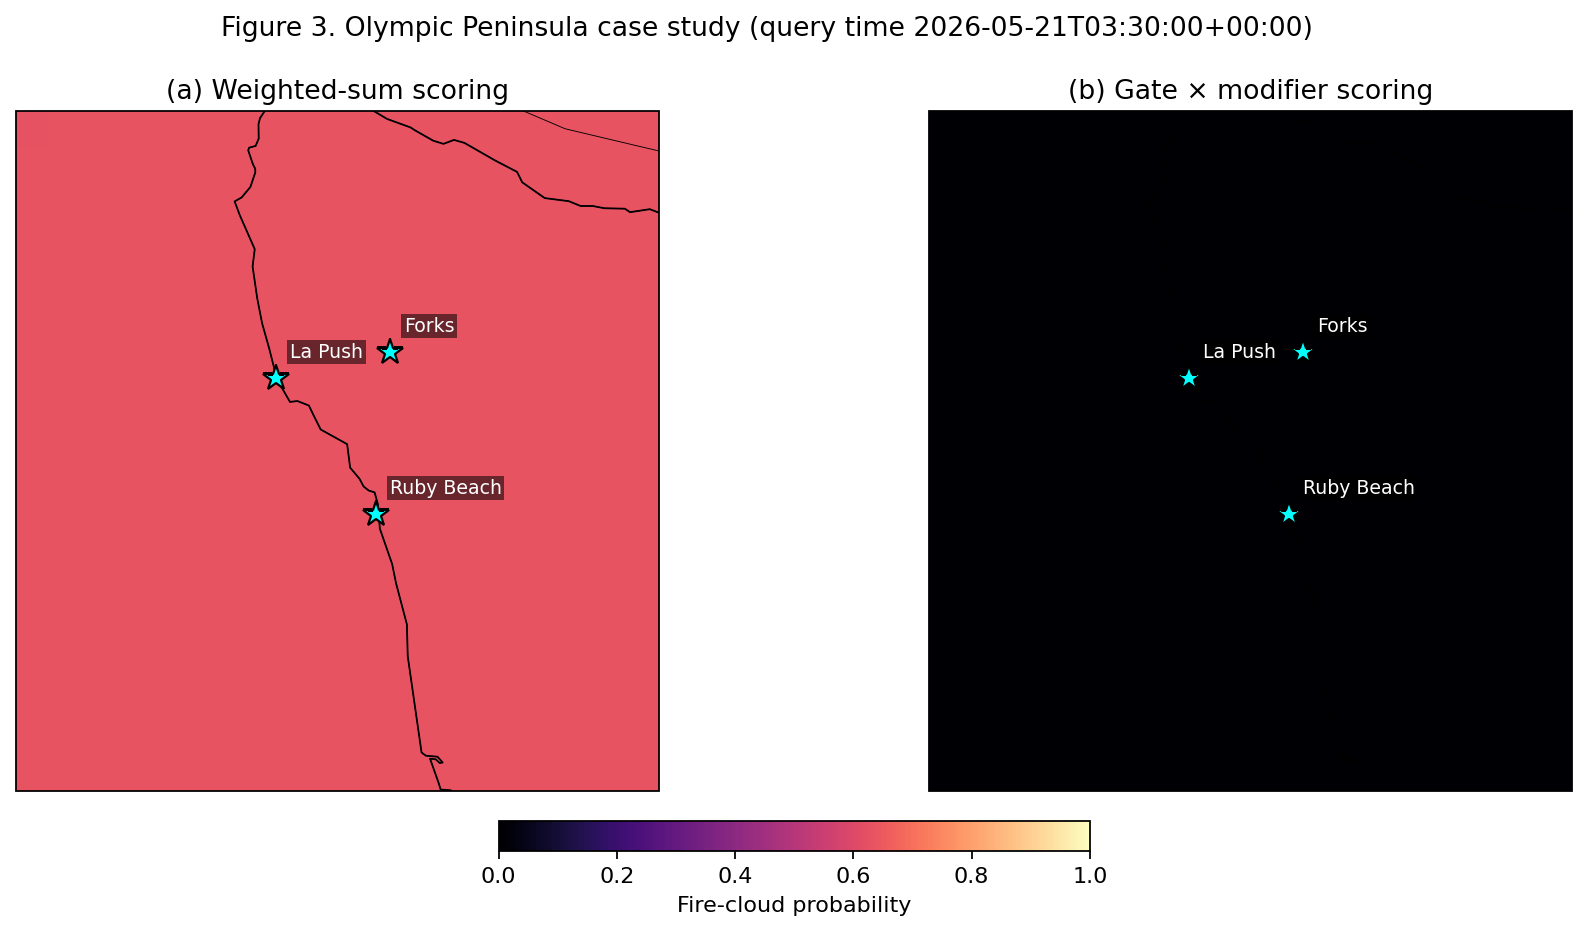
\includegraphics[width=\linewidth]{fig3_olympic_peninsula.png}
\caption{Olympic Peninsula case study comparing weighted-sum scoring (\textbf{left}, current implementation) against the proposed gate $\times$ modifier scoring (\textbf{right}, this paper). Both panels use the same per-rule component scores computed from a single HRRR forecast cycle (initialized 01:00 UTC on 21 May 2026, forecast hour 2). Cyan stars mark La Push, Forks, and Ruby Beach. The weighted-sum panel returns 0.625--0.631 across all 180 grid cells despite zero HRRR-reported mid- and high-cloud coverage; the gate $\times$ modifier panel returns 0.000 in every cell.}
\label{fig:olympic}
\end{figure}

\subsection{Sensitivity and Limitations}
\label{sec:limitations}

This case study is not a validation: we do not have ground-truth observations of whether a glow actually occurred at Forks on the queried evening. (The HRRR-reported atmospheric state, with zero mid and high cloud cover, suggests no glow was possible.) We use the case study only to demonstrate the structural failure mode of weighted-sum scoring and the corrective behavior of the gate $\times$ modifier alternative. Statistical validation against citizen-science ground truth is the subject of planned future work (Section~\ref{sec:validation}).

Two implementation issues surfaced during this case study and have been addressed in the current code:
\begin{enumerate}
\item \textbf{Serial loop re-parsing HRRR data.} A naive \texttt{HRRRSource.fetch} re-instantiates Herbie and re-parses GRIB2 via cfgrib for every query, introducing roughly ten minutes of redundant work per 150-point notebook run. We mitigate with the per-instance in-memory dataset cache (Section~\ref{sec:code}).
\item \textbf{Cosine-latitude correction.} The HRRR grid is Lambert Conformal with two-dimensional latitude--longitude arrays. A naive Euclidean nearest-neighbor in raw degrees ignores the $\cos\phi$ compression and, at the Olympic Peninsula's $48^\circ$\,N, can select a grid cell whose ground distance is up to one cell (3\,km) farther than the true nearest. We apply Eq.~\ref{eq:coslat}.
\end{enumerate}
Both are tested explicitly in the test suite.

\section{Discussion}
\label{sec:discussion}

\subsection{Implications for Atmospheric Science}

The gate $\times$ modifier framework is not specific to sunset glow prediction. It applies whenever an outcome depends on the conjunction of multiple physically necessary conditions, none of which can be substituted by another. Several operational forecasting problems fit this pattern:
\begin{itemize}
\item \textbf{Convective storm initiation} requires the simultaneous presence of conditional instability (positive CAPE), a lifting mechanism (a trigger such as a front or convergence line), and adequate low-level moisture.
\item \textbf{Aurora visibility from a given ground location} requires geomagnetic activity above a threshold, clear local sky, and astronomical darkness.
\item \textbf{Stratospheric ozone hole formation} requires polar stratospheric clouds (cold), reactive halogen species (chlorine and bromine), and returning spring sunlight.
\end{itemize}
Operational forecasting heuristics in each of these domains commonly express conditions through weighted indices or color-coded thresholds that, on inspection, treat necessary conditions additively. The gate $\times$ modifier separation we develop here is a small architectural change with potentially wide applicability when the underlying phenomenon has AND-gated necessary causes.

\subsection{Comparison with Existing Services}

SunsetWx and Sunsethue both publish enough information about their methodologies to permit qualitative reconstruction. SunsetWx's public summary \citep{forecastingbeauty2015} describes a ``20-factor algorithm'' using GFS data with cloud cover, moisture, and pressure as core factors and a final weighted score; the language is suggestive of additive composition without explicit gating. Sunsethue's blog narrative similarly lists factor ranges without distinguishing necessary from enhancing conditions. Closed-source services such as Skyfire publish even less.

We do not have systematic ground-truth comparisons against these services. The case study of Section~\ref{sec:casestudy} demonstrates only that \emph{our own} prior weighted-sum implementation produced a clearly false positive in a configuration that no physically motivated predictor should classify as favorable; we cannot extend the demonstration to SunsetWx or Sunsethue without access to their internals or a paired-prediction dataset with ground truth.

\subsection{Open Questions and Limitations}
\label{sec:openquestions}

\begin{enumerate}
\item \textbf{Operational ozone column data are not real-time.} NASA OMI and TROPOMI products are produced on a daily cadence with one-to-several-day latency. Incorporating the Chappuis modifier requires either tolerating a stale TOC input or supplementing satellite retrievals with an operational model.
\item \textbf{Aerosol layer separation is not directly observable from HRRR.} Distinguishing stratospheric from tropospheric aerosol contributions requires satellite limb-sounding products such as OSIRIS or OMPS-LP.
\item \textbf{Choice of scoring-function shape.} We use trapezoidal and piecewise-linear forms for interpretability. Smoother forms (Gaussian, sigmoid, beta) would produce continuously differentiable predictors but introduce hyperparameters whose principled fitting requires labeled data.
\item \textbf{No formal sensitivity analysis.} The case study is qualitative. A systematic analysis of the composite probability to each rule's parameters across a large grid of synthetic inputs would strengthen confidence and is identified as future work.
\item \textbf{The Olympic Peninsula case study is not a validation.} We demonstrate a failure mode of weighted-sum scoring in a configuration where physical reasoning predicts no glow, but we have not collected the observation that would confirm no glow occurred.
\item \textbf{HRRR-Smoke is CONUS-only.} Wildfire-driven aerosol enhancement, operationally important in Pacific Northwest and California fire seasons, is captured by HRRR-Smoke but unavailable outside the HRRR domain.
\end{enumerate}

\subsection{A Taxonomy of NWP-Driven Forecast Failure Modes}
\label{sec:failuremodes}

A separate class of limitations stems not from the predictor's design but from uncertainty in the upstream NWP forecast. When a fire-cloud prediction proves wrong (a so-called ``forecast bust''), it is operationally useful to characterize the failure with specific physical language rather than blanket statements like ``too cloudy'' or ``too hazy.'' The operational workflow of Section~\ref{sec:workflow} surfaces several distinct failure modes worth flagging when characterizing prediction uncertainty:

\begin{enumerate}
\item \textbf{Cloud-amount uncertainty within the layer.} A relatively-humid layer in the NWP cross section is predicted to be cloudy at the threshold (e.g., RH $\approx 90\%$). If the actual humidity is a few percent lower, the cloud may not form at all. This failure is most acute when the predicted cloud layer is thin and the RH peak within it just barely exceeds saturation.
\item \textbf{Cloud-boundary position uncertainty.} The horizontal position of the cloud's edge along the sunset direction depends on the spatial gradient of the moisture field, which itself depends on the NWP forecast's accuracy. A relative-humidity field that drops gradually from 95\% to 85\% over 100\,km has a much less certain ``cloud edge'' than one that drops from 99\% to 1\% over 1\,km. Modest forecast biases in the gradual case produce large shifts in cloud boundary location.
\item \textbf{Cloud-edge wind speed.} Even if the boundary's location is well predicted, the wind speed component along the sunset direction at the cloud's altitude controls how quickly the boundary translates between the NWP analysis time and the actual sunset moment. Empirically, an along-direction wind component below 15~m/s introduces small position uncertainty; 15--30~m/s introduces moderate uncertainty; above 30~m/s introduces large uncertainty, with the cloud potentially translating tens of kilometers between successive NWP outputs.
\item \textbf{Small angle between cloud boundary and sunset direction.} When the cloud's edge is nearly parallel to the sunset azimuth, a small lateral shift in either the cloud edge or the solar azimuth produces a large shift in the cross-section's cloud-edge position. Such configurations carry intrinsically high uncertainty; rules of thumb suggest care when the angle between cloud-edge tangent and sunset azimuth falls below $10^\circ$.
\item \textbf{Unaccounted intervening clouds.} The geometric model treats the sunset light path as obstructed only by Earth's shadow and the target cloud's own boundary. In practice, additional mid- or low-level cloud layers between the observer and the target cloud can intercept the light path. Inspection of the full vertical cross section, not just the target cloud's altitude, is required.
\item \textbf{Upstream aerosol underestimation.} The aerosol forecast (HRRR-Smoke or equivalent) reflects \emph{local} aerosol concentration; the relevant quantity for fire-cloud color is the aerosol along the upstream sunlight path, which may span hundreds of kilometers in the sunset direction. A clean local atmosphere does not guarantee a clean upstream path. This is the most subtle of the failure modes and is captured imperfectly even with high-resolution aerosol forecasts.
\end{enumerate}

A forecaster reviewing a busted prediction should be able to attribute the failure to a specific item in this list rather than a generic ``the model was wrong.'' Operationally this discipline yields better calibration of future forecasts and a more honest accounting of prediction uncertainty.

\section{Conclusion and Future Work}
\label{sec:conclusion}

\subsection{Summary}

We have presented a physics-motivated framework for sunset glow prediction over the continental United States, with three principal contributions. First, an explicit catalog of necessary versus enhancing atmospheric conditions for the phenomenon, grounded in peer-reviewed atmospheric optics literature including the recent \citet{lange2023revisiting} refinement that ozone Chappuis absorption dominates twilight sky color at low solar elevations. Second, a two-layer gate $\times$ modifier scoring architecture that respects the multiplicatively-gated nature of necessary conditions and avoids a class of false positives produced by weighted-sum scoring as used in existing commercial services. Third, an open-source Python implementation consuming NOAA HRRR data with end-to-end reproducibility. A preliminary case study on the Olympic Peninsula demonstrates the structural failure mode of weighted-sum scoring (probability $\sim 0.63$ in a configuration with zero mid- and high-level cloud) and the corrective behavior of the gate $\times$ modifier architecture (probability $\to 0$ in the same configuration). Full validation against ground-truth observations is identified as the principal piece of remaining work before peer-reviewed submission.

\subsection{Citizen-Science Validation Pipeline}
\label{sec:validation}

A statistically meaningful validation of any sunset prediction algorithm requires paired (prediction, observation) records over a wide range of conditions and locations. We propose a citizen-science observation pipeline as the cheapest path to such a dataset.

The pipeline has three components: a structured observation submission interface, a calibration step against expert reference observations, and a statistical methodology for handling observer bias and geographic non-uniformity. Structured submissions would record date, time, location, a five-point visual rating of glow intensity, a controlled color vocabulary, qualitative cloud type/coverage estimates, and a photograph for spot-check verification. Integration with an existing platform such as iNaturalist would lower onboarding friction at the cost of less structured data; a dedicated portal would invert the tradeoff.

Even modest data volumes are sufficient to evaluate the framework's qualitative pathology fix: a hundred paired records over a few weeks would suffice to test whether the gate $\times$ modifier predictor's high-probability outputs correspond to observed glows more reliably than weighted-sum outputs. Larger volumes would support fitted weight optimization (Section~\ref{sec:mlext}) and geographic generalization studies.

\subsection{Machine Learning Extension}
\label{sec:mlext}

Once a labeled dataset exists, the \texttt{Predictor} Protocol allows a drop-in \texttt{MLPredictor} implementation consuming the same \texttt{Features} representation as \texttt{RuleBasedPredictor}. Several model families are appropriate: gradient-boosted decision trees (XGBoost, LightGBM) on the existing feature set offer interpretable feature-importance reports; logistic or beta regression yields probability outputs with calibration properties suited to forecasting use; feed-forward neural networks become viable at larger training volumes.

In all cases the rule-based predictor functions as an interpretable baseline against which ML accuracy gains are measured. A separate research direction is \emph{color} prediction: \citet{lange2023revisiting}'s ozone column dependence suggests that color (red vs.\ orange vs.\ purple) is itself predictable from atmospheric inputs, a regression target not attempted by any existing service.

\subsection{Global Expansion}
\label{sec:globalext}
\label{sec:future}

The HRRR-based predictor described here is operational only for the continental United States. Global coverage requires substitution of the \texttt{WeatherSource} implementation with one consuming GFS (at $0.25^\circ$ resolution). The change is mechanically straightforward but the physical implications include reduced spatial resolution and loss of the HRRR-Smoke wildfire aerosol product. For regions where higher-resolution regional models exist (UK Met Office UKV, European COSMO-DE, Chinese CMA-GD), domain-specific \texttt{WeatherSource} implementations would restore HRRR-equivalent resolution at the cost of additional engineering effort.

\section*{Acknowledgments}

The geometric reformulations of Sections~\ref{sec:parabola}--\ref{sec:triangle} (the parabolic light-path approximation, the fire-cloud spatiotemporal triangle, the equivalent-cloud-base correction for atmospheric extinction) and the operational workflow of Section~\ref{sec:workflow} draw on an extensive Chinese-language community knowledge base on amateur sunset-cloud forecasting in the Yangtze Delta region, which compiles operational meteorological practice not otherwise published in the peer-reviewed literature. The framing of forecast-failure modes in Section~\ref{sec:failuremodes} similarly reflects practitioner consensus from that community.

[Additional acknowledgments to be added in camera-ready version.]

\bibliography{references}

\appendix

\section{Rule Weights and Parameters}

To be added: a complete table of all \texttt{ScoringRule} parameters in the current implementation, their values, and the literature anchor for each.

\section{Code Listings}

To be added: minimal code excerpts showing the \texttt{Predictor} protocol, the \texttt{RuleBasedPredictor.score} method, and the \texttt{gate\_modifier\_combiner} function.

\end{document}
